\documentclass{article}
\usepackage{graphicx}
\title{Write-up 1}
\author{Luojie Xiang}
\date{}

\begin{document}

\maketitle

\section{Already Implemented Modules}
The following is the already implemented modules:

\begin{itemize}
\item WLZW 

LZW is a lossless data compression algorithm. It builds a dictionary during the compression process. This dictionary contains frequent patterns in the text being compressed. Our interest is in extracting frequent patterns out of text, so a LZW algorithm is applied and the dictionary is stored for future use (such as pattern frequency estimation). 

LZW works on character level but we are only interested in patterns on word level. Therefore, the original LZW algorithm is modified to work on world level (WLZW). Furthermore, we don't want patterns that span across sentences. NLTK is used to split a chunk of text into sentences and WLZW is applied sentence by sentence. Despite the sequential nature of LZW algorithm, when a text is large enough, it can be splitted into smaller chunks and a WLZW is run on each of them. At a final step, all output dictionaries are unioned together. In this way, WLZW is parallelized. Currently only shared memory model is implemented.

\item Aho-Corasick algorithm

Aho-Corasick algorithm is a string searching algorithm that constuct a finite state machine using a finite dictionary and do a linear scan through the input text to match the strings in the dictionary. Aho-Corasick algorithm is used to match and thus estimate the frequencies of patterns extracted from the WLZW algorithm.

An open source implementation of Aho-Corasick algorithm is found, Acora. However, it matches on character level. It is thus wrapped up such that only matches that are on the word level is kept and the frequency of each pattern is counted.

\end{itemize}
\section{Modules To Be Implemented}
Following is the moduels that are being implemented or to be implemented in the future:

\begin{itemize}
\item Importance Estimation

The frequent patterns extracted from previous modules needs to be ranked by their importance. Three metrics is going to be implemented: TF-IDF, MI, RIDF.

\item SQLite wrapper
 
In order to compute the importance estimations, frequent patterns and their corresponding information needs to be precomputed. These information need to be stored so that they could be efficiently retrieved later. Thus a SQLite wrapper is needed to query data in python.

\item Support of parallel computation

Both distributed and shared memory model needs to be supported and user should have the freedom to choose which model to use.

\item Documentation and testing

Good documentation needs to be written and generated for future development of the project. Furthermore, the developed modules needs to be tested on both Linux and Windows. Performance needs to be measured on different datasets.

\end{itemize}

\section{Performance Measure}

The following tests the shared memory model parallelization of WLZW.

Experiment setup:
ocean1.cs.purdue.edu 32 cpu 

On kb.txt (24MB, 4,749 lines, 3,232,894 words, 24,467,795 characters)

\begin{tabular}{|l|l|}
\hline
\# processes &time (s) \\
\hline
1&  21.83 \\
\hline
2&  11.43 \\
\hline
4&  6.68 \\
\hline
8&  4.45 \\
\hline
16&  4.00 \\
\hline
32&  4.97 \\
\hline
\end{tabular}

On tweets (70MB, 1,000,000 lines, 12,202,377 words, 73,356,788 characters)

\begin{tabular}{|l|l|}
\hline
\# processes& time (s) \\
\hline
1&  86.79  \\
\hline
2&  52.04 \\
\hline
4&  32.85 \\
\hline
8&  26.01 \\
\hline
16&  23.89 \\
\hline
32&  31.18 \\
\hline
\end{tabular}

The run time decreases until 32 processes is used. The reason why run time increases after that is the union of patterns from different processes dominates the run time. The results from the above two tables are shown in Fig. \ref{time}.

\begin{figure}
\centering
\label{time}
\caption{Performance of Parallel WLZW module}
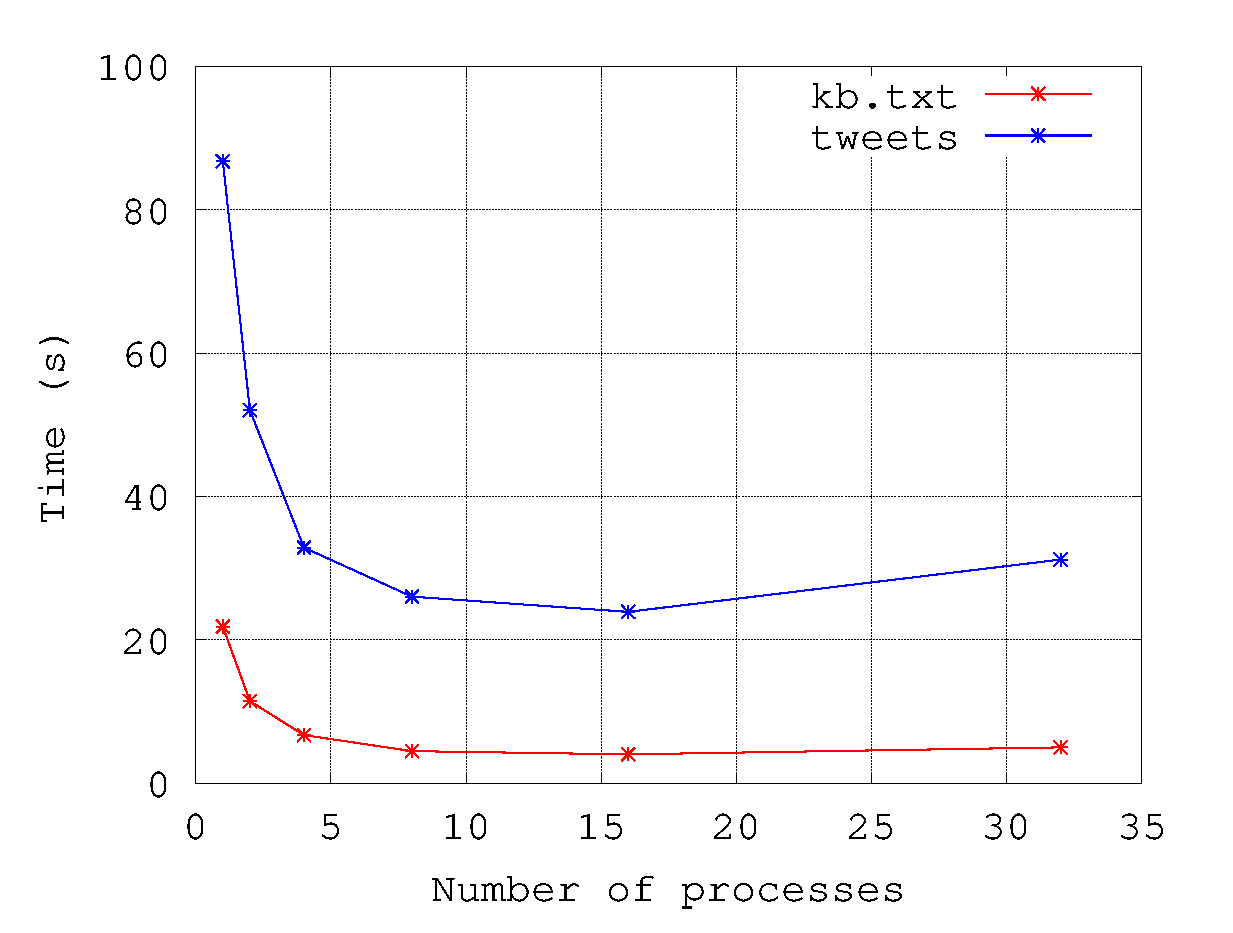
\includegraphics[width=0.8\textwidth]{time}
\end{figure}

The Aho-Corasick algorithm's performance will be tested in the future along with the importance ranking modules.

\end{document}

